\section{Исследовательская часть}

В данном разделе представлены результаты исследований, проведённых для оценки производительности системы при увеличении объёма данных, анализа скорости получения ответа в зависимости от количества одновременных запросов, а также сравнения скорости обработки с использованием кэширования и без него.

\subsection{Технические характеристики}

Исследования проводилось на устройстве со следующими техническими характеристиками:

\begin{itemize}[label=---]
	\item операционная система macOS 14.6.1~\cite{macos};
	
	\item оперативная память (RAM) 16 ГБ;
	
	\item процессор (CPU) 2 ГГц 4‑ядерный Intel Core i5 (8 логических ядер)~\cite{intel}.
	
\end{itemize}

Во время проведения исследования, устройство было подключено к сети электропитания и не было нагружено сторонними приложениями, за исключением встроенных приложений окружения.

\subsubsection*{\normalsize  Влияние объема данных на время выполнения}


В таблице~\ref{tab:user_performance} представлены усреднённые значения исследования времени выполнения операций INSERT, SELECT, UPDATE и DELETE в зависимости от количества строк в таблице User. Измерения проводились при объёмах данных от 100 до 99{,}1000 записей с шагом 1{,}000. Для каждой операции выполнялось 10 повторений, после чего вычислялось среднее время выполнения одной операции в миллисекундах.

На рисунке~\ref{grp:dr} приведена диаграмма, иллюстрирующая зависимость времени выполнения каждой операции от размера таблицы.

В приложении A приведены листинги кода, использованные при проведении исследования производительности операций INSERT, SELECT, UPDATE и DELETE на таблице User.

\newpage
\begin{table}[ht]
	\centering
	\caption{Среднее время операций с таблицей \texttt{User} (в миллисекундах)}
	\begin{tabular}{|r|r|r|r|r|}
		\hline
		Размер таблицы & INSERT & SELECT & UPDATE & DELETE \\
		\hline
		100   & 0.0166 & 0.0325  & 0.0396  & 0.0307  \\
		1100   & 0.0183  & 0.2800 & 0.1231  & 0.0951  \\
		5100   & 0.0332 & 1.1239  & 0.5739  & 0.0871  \\
		10100   & 0.0449  & 2.6399  & 1.1599  & 0.9866  \\
		25100  &0.0670  & 11.6802 & 6.0323  & 5.2592  \\
		50100  & 0.0637  & 14.2658  & 5.6018  & 6.1221 \\
		99100 & 0.0758  & 23.2923  &9.3653  & 9.3532 \\
		\hline
	\end{tabular}
	\label{tab:user_performance}
\end{table}

\begin{figure}[ht!]
	\begin{center}
		\begin{tikzpicture}
			\begin{axis}[
				legend pos = north west,
				xlabel=размер таблицы,
				ylabel=секунды,
				grid = major,
				major grid style = {lightgray},
				minor grid style = {lightgray!25},
				width = 1.0\textwidth,
				height = 0.7\textwidth,
				scaled y ticks=base 10:0,
				]
				
				\addplot[
				purple,
				semithick,
				mark = o,
				] file {./diag/delete.txt};
				\addlegendentry{DELETE}
				
				\addplot[
				red,
				semithick,
				mark = +,
				] file {./diag/insert.txt};
				\addlegendentry{INSERT}
				
				\addplot[
				blue,
				semithick,
				mark = *,
				] file {./diag/update.txt};
				\addlegendentry{UPDATE}
				
				\addplot[
				darkgray,
				semithick,
				mark = x,
				] file {./diag/select.txt};
				\addlegendentry{SELECT}
			\end{axis}
		\end{tikzpicture}
	\end{center}
	\caption{Зависимость времени выполнения операций от записей в таблице}
	\label{grp:dr}
\end{figure}

\subsubsection*{\normalsize Вывод}

 Полученные результаты (в миллисекундах) показали следующее:

\begin{itemize}
	\item \textbf{INSERT} -- время выполнения увеличилось с 0.0167 мс при 100 записях до 0.0758 мс при 99 100 записях -- рост на \(\approx354\%\);
	\item \textbf{SELECT} -- время выполнения увеличилось с 0.0325 мс до 23.2923 мс -- рост более чем на \(71\,500\%\);
	\item \textbf{UPDATE} -- время выполнения увеличилось с 0.0396 мс до 9.3653 мс -- рост примерно на \(23\,600\%\);
	\item \textbf{DELETE} -- время выполнения увеличилось  с 0.0307 мс до 9.3532 мс -- рост на \(30\,400\%\).
\end{itemize}

Таким образом, при увеличении объёма данных операции \textit{SELECT}, \textit{UPDATE} и \textit{DELETE} оказываются примерно в одинаковой мере медленнее по сравнению с \textit{INSERT}, который сохраняет относительную быстроту даже при больших объёмах.

В результате серии измерений были выявлены единичные <<пики>> задержек при выполнении операций. Такие выбросы обусловлены не ростом сложности самого запроса, а фоновой активностью СУБД и операционной системы.

\subsubsection*{\normalsize Влияние количества одновременных запросов на отклик}

В таблице~\ref{operation-times2} приведены результаты исследования времени отклика от количества клиентов в миллисекундах в течение 10 секунд. На рисунке~\ref{grp:dr2} изображено графическое представление данных из таблицы~\ref{operation-times2}.

На листинге~\ref{lst:select_gender} приведён SQL-запрос, используемый для измерения времени отклика.

\begin{table}[h!]
	\centering
	\caption{Результаты нагрузочного исследования}
	\begin{tabular}{|p{3.5cm}|p{4.5cm}|p{3.5cm}|}
		\hline
		\textbf{Количество клиентов} & \textbf{Среднее время отклика (мс)} & \textbf{Количество запросов} \\
		\hline
		1  & 0.272817  & 36\,550 \\
		10 & 1.516456  & 65\,898 \\
		25 & 5.964658  & 41\,914 \\
		50 & 11.333167 & 44\,124 \\
		75 & 13.321161 & 56\,332 \\
		\hline
	\end{tabular}
	\label{operation-times2}
\end{table}

\newpage
\begin{lstlisting}[language=SQL,
	label=lst:select_gender,
	caption={Извлечение данных о пользователях мужского пола} ,
	captionpos=t,
	basicstyle=\ttfamily\small]
SELECT * 
FROM "User" 
WHERE gender = 'мужской';
\end{lstlisting}

\begin{figure}[ht!]
	\begin{center}
		\begin{tikzpicture}
			\begin{axis}[
				legend pos = north west,
				xlabel=количество клиентов,
				xmin=-1,
				xmax=77,
				ylabel=миллисекунды,
				grid = major,
				major grid style = {lightgray},
				minor grid style = {lightgray!25},
				width = 1.0\textwidth,
				height = 0.5\textwidth,
				scaled y ticks=base 10:0,
				]
				
				\addplot[
				purple,
				semithick,
				mark = o,
				] file {./diag/time-avg-results.txt};
			\end{axis}
		\end{tikzpicture}
	\end{center}
	\caption{Зависимость времени отклика от количества клиентов}
	\label{grp:dr2}
\end{figure}

\subsubsection*{\normalsize Вывод}

Результаты второго исследования показали, что с увеличением количества клиентов время отклика на запросы также увеличивается. Так, при 10 клиентах среднее время отклика составило 1.5165 мс, а при 75 клиентах -- 13.3212 мс. Это свидетельствует о том, что с ростом числа одновременных запросов наблюдается значительное увеличение времени отклика, что указывает на увеличение нагрузки на базу данных.

\subsubsection*{\normalsize Влияние кэширования на скорость запросов}

В рамках исследования была оценена производительность запросов к данным, получаемым из базы данных PostgreSQL и Redis-кэша. 

В данном исследовании для оценки скорости выборки из PostgreSQL и Redis-кэша использовался SQL-запрос, представленный на листинге \ref{lst:select_redis}.

\begin{lstlisting}[language=SQL,
	label=lst:select_redis,
	caption={Извлечение данных о пользователях женского пола, рождённых после 1 января 2003 г., с сортировкой по дате рождения},
	captionpos=t,
	basicstyle=\ttfamily\small]
SELECT * FROM "User" u
JOIN "Membership" m on m.user_id = u.id
JOIN "Order" o on o.id = m.order_id
WHERE birth_date > '2003-01-01' AND gender = 'женский'
ORDER BY birth_date DESC;
\end{lstlisting}

Для каждого из источников данных были замерены времена отклика на запросы. Каждый запрос к кэшу и базе данных выполнялся 30 раз. Исследование проводилось на протяжении нескольких минут, с интервалом в 5 секунд между запросами. Кэш в Redis хранился в течение 10 секунд.

Среднее время выполнения запросов к Redis-кэшу (Кэш) составило 0.00188 секунды, для базы данных PostgreSQL (БД) -- 0.00246 секунды. На рисунке~\ref{fig:dr3} изображено графическое представление полученных данных. 

\begin{figure}[ht!]
	\begin{center}
		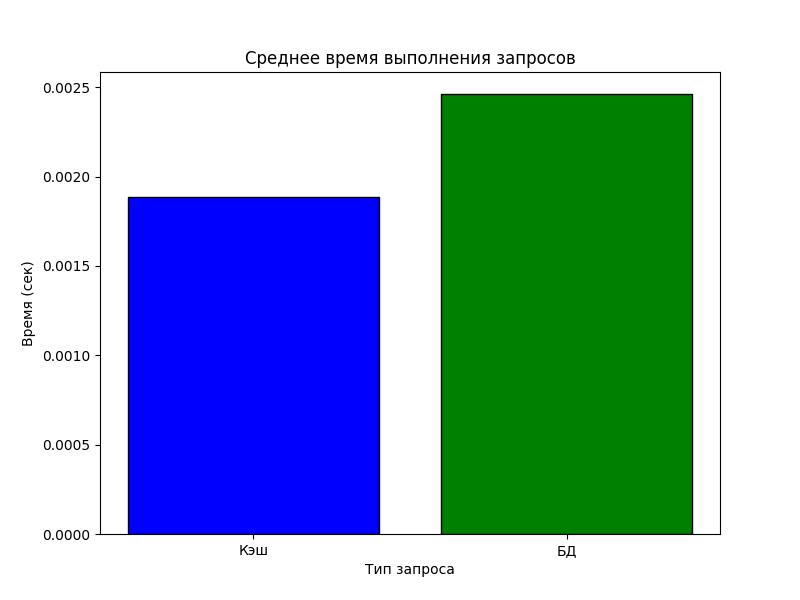
\includegraphics[scale=0.7]{./img/just.png}
	\end{center}
	\caption{Сравнение времени выполнения запросов к кэшу и базе данных}
	\label{fig:dr3}
\end{figure}


\subsubsection*{\normalsize Вывод}

Результаты третьего исследования показали, что кэширование ускоряет выполнение запросов. Среднее время выполнения запроса к Redis-кэшу составило 0.00188 секунды, что на 0.00058 секунды быстрее, чем запросы к базе данных PostgreSQL, где среднее время составило 0.00246 секунды. Это подтверждает эффективность использования кэширования для ускорения обработки данных.